
The proposed FVR method is interesting in comparison with other major techniques, such as Feature Matching + RANSAC, ICP and other optimization methods, in that it is a closed form solution and not an iterative solution. That is, its computational complexity is fixed and does not depend on the input data. Despite this, some parts of the pipeline (see Figure \ref{fig:PIPELINENo1}) remain intensive, even for GPGPU and other parallel processing devices. \\

To reduce complexity, the different parts of the pipeline were examined to reveal any possible improvements. It is understood that each Hanning window function in Figure \ref{fig:PIPELINENo1} is required to reduce noise on the phase correlation surface. The technique is already highly parallelized and is not very computationally intensive. Much effort has also already been given to improving efficiency in computing the Fourier transform. \\

The element-wise log function is similar to the Hanning window function, it is required to correlate the data to find the rotation and scale factors separating both volumes. Furthermore it is already highly parallelized and cannot be simplified. The 3D phase correlation technique is by far the most computationally intensive operation within the pipeline. It requires 2 $\times$ FFTs, 1 $\times$ element-wise operation, 1 $\times$ inverse FFT and 1 $\times$ peak search operation. Moreover, there are two required 3D phase correlation operations during the pipeline. The other transform operations are also element-wise operations introducing minimal computation expense into the pipeline. \\

To reduce the computational complexity of the 3D phase correlation, several projection operations are used to retain as much information as possible whilst reducing the data to 2 dimensions in such a way that 2D phase correlation (a much faster operation) may be used in place of 3D phase correlation to retrieve transformation factors. Two transforms are proposed to achieve this. The Spherical-Map Transform (section \ref{SMTransform}) reduces the original 3D frames to 2D. One useful property of this transformation is that correlation between two Spherical-Map domains retrieved from two 3D frames yields the y-axis rotation and scale factor parameters between the original 3D frames. Moreover, because the spherical-map space is a 2D space, phase correlation may be used in place of manual correlation.  \\

The other transformation is proposed to efficiently compute translation factors separating two 3D volumes. This transform is simply named a projection transform (see section \ref{sec:PMTramsform}). It reduces the 3D input frames to 2D images whilst retaining the translational information along two remaining axes. Correlating two projection transform domain images yields two translation parameters (depending on the type of projection transform) which separate the two original 3D frames. \\

A block diagram integrating these speed improvements into the FVR method introduced in section \ref{FVRSectionA} is shown in Figure \ref{fig:PIPELINE3}. This procedure is referred to as the Fast Fourier Volume Reconstruction method (FFVR). As shown in the block diagram, this procedure takes two 3D volume frames as input, $Volume_1$ and $Volume_2$. The second frame may be taken after the camera has changed pose about the y-axis and/or has moved locations. Both inputs are then put through a 3D FFT function to produce the magnitude values of the 3D frequency domain of both volumes. These operations may be performed on a GPGPU and may be performed in parallel with each other. \\

The magnitude of the frequency domain is independent of translation and any rotation and scale occurs about the centre of both volumes. Both frequency domain volumes are then transformed into 2D spherical space using the $Spherical2DMap$ function. This function produces an image in which 3D y-axis rotation from the original volume is interpreted as 2D translation. To recover the rotation parameter, phase correlation is used to measure the translational component separating the spherical-map domain images. This translational component is then processed to compute the y-axis rotational factor separating the original input volumes. The rotation factor can be directly output as a parameter if required. \\


\begin{figure}[!h]
\centering
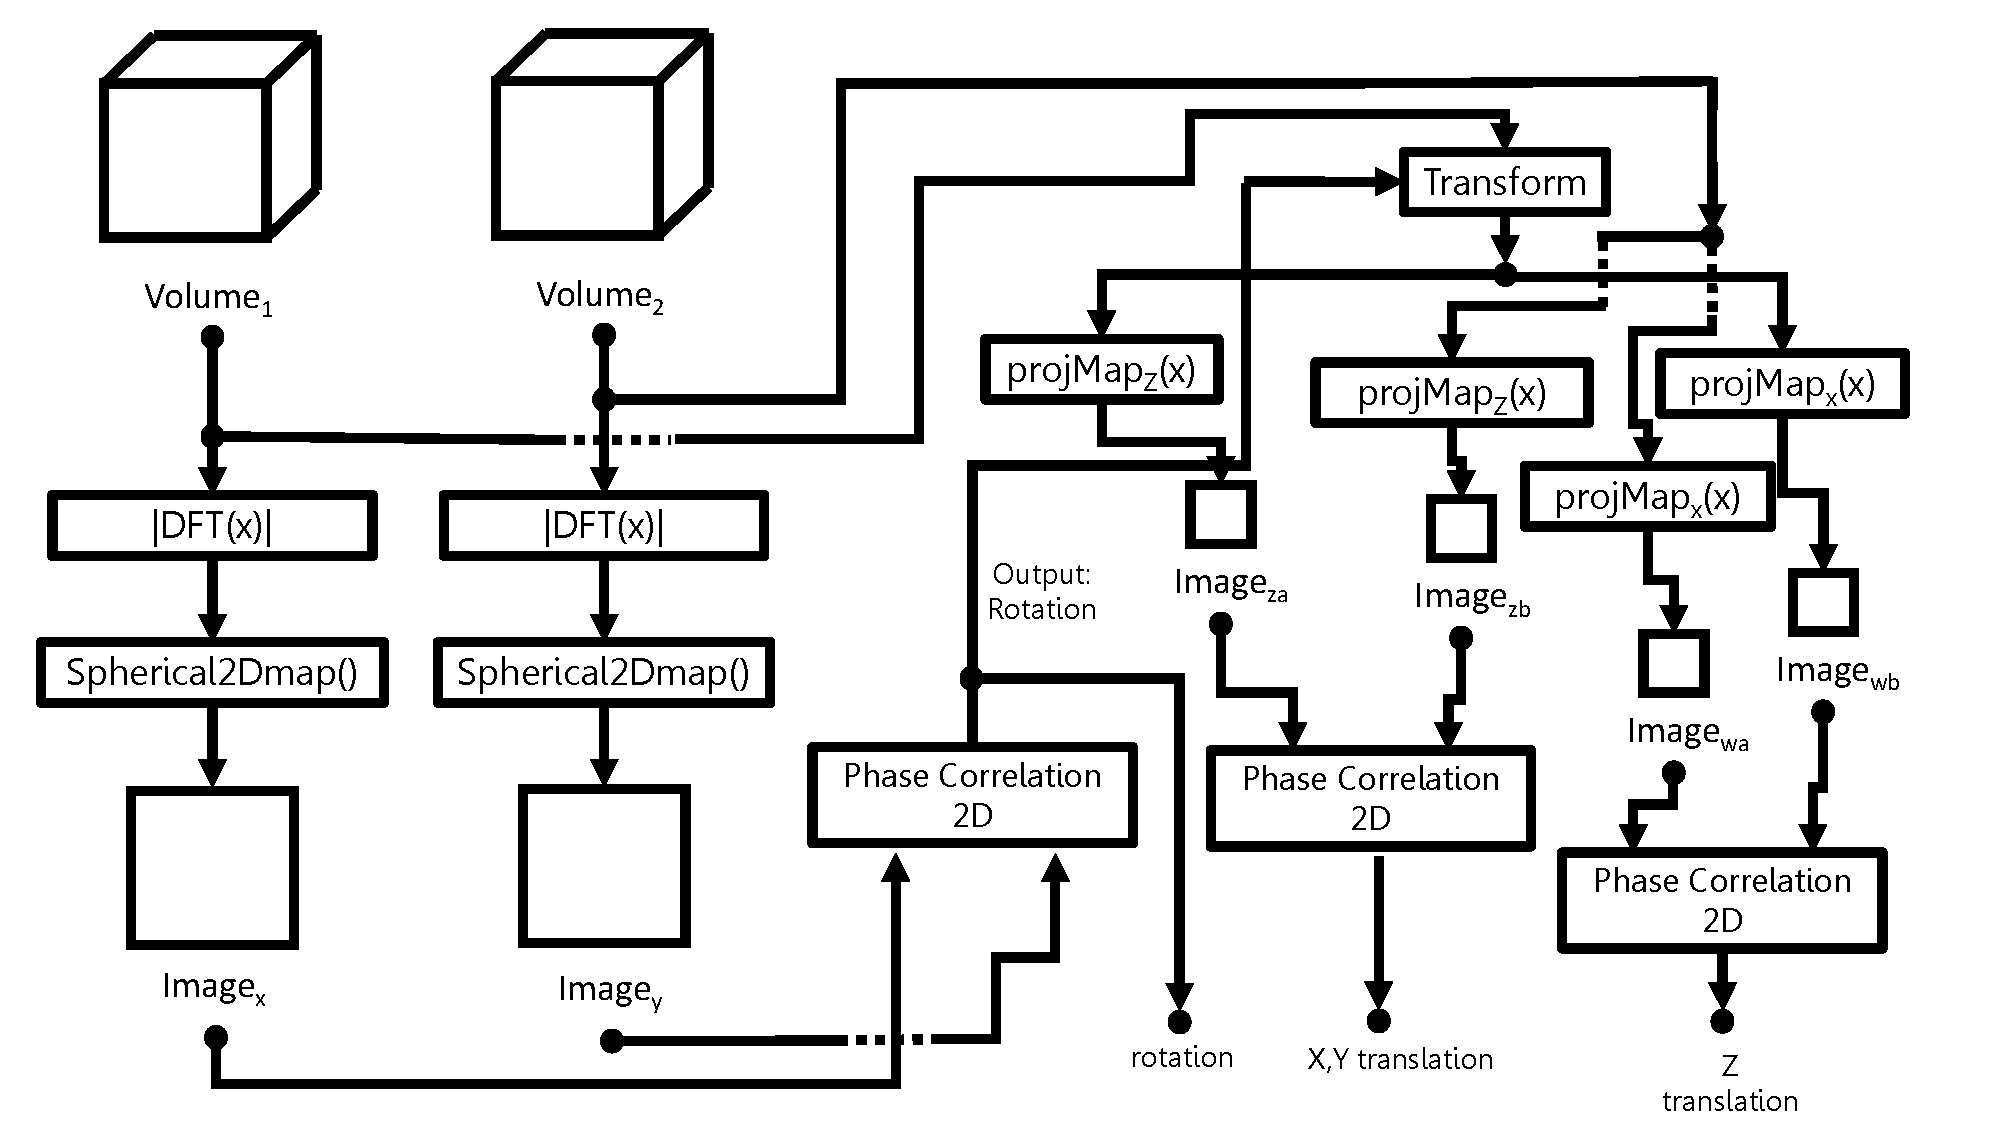
\includegraphics[width=5.0in]{images/ch2/pipeline3}
\caption{System Diagram for Fast Volume Registration}
\label{fig:PIPELINE3}
\end{figure}

Next, the first 3D frame, $Volume_1$ is transformed by the computed rotation factor. This leaves only a 3D translation transform separating both inputs $Volume_1$ and $Volume_2$. Two Projection-map transforms of both $Volume_1$ and $Volume_2$ (equivalent to four transforms in total) are then used to efficiently find this translation factor. The first Projection-map transform is along the z-axis. The z-axis Projection-map transform of $Volume_1$ produces 2D image, $Image_{za}$ the z-axis Projection-map transform of $Volume_2$ produces 2D image, $Image_{zb}$. Both $Image_{za}$ and $Image_{zb}$ may be phase correlated producing the x and y axis components of the translation separating $Volume_1$ and $Volume_2$. \\

The other two Projection-map transforms are along the x-axis. The Projection-map transform of $Volume_1$ produces $Image_{wa}$, whilst the Projection-map transform of $Volume_2$ produces $Image_{wb}$. These two images ($Image_{wa}$ and $Image_{wb}$) may be phase correlated producing the z-axis component of the translation. A composite registration matrix aligning $Volume_1$ to $Volume_2$ may be formed by translating each volume's centre to the origin, rotating by the computed rotation factor, translating the origin to the volume's centre and finally translating by the $[X,Y,Z]^T$ translation vector computed. \\

Noticeably, the Hanning window function and post $|DFT|(x)$ $Log(x)$ function from the original pipeline (figure \ref{fig:PIPELINENo1}) are missing. The Hanning window function may be incorporated in the first phase correlation procedure, which processes 2D images, therefore the Hanning window function would be in 2D rather than 3D which also improves efficiency as an entire dimension is removed from the process. The log function may also be performed as part of the phase correlation procedure, however it was found that the FFVR procedure estimates rotation more reliably using the spherical-transform if the log function is not performed. Consequentially, this saves computational cost. \\

It is advantageous to use 2D phase correlation over 3D phase correlation from a computational complexity perspective. The 3D Fourier transform has complexity of $N^3 \times Log(N^3)$ whilst the 2D has complexity $N^2 \times Log(N^2)$. Essentially the amount of data to process has been reduced by an entire dimension. The phase correlation method requires 2 $\times$ FFTs, 2 $\times$ element-wise computations and 1 $\times$ inverse FFT. The corresponding 3D phase correlation complexity equates to $3N^3Log(N^3) + 2N^3$ whilst the 2D equivalent is only $3N^2Log(N^2) + 2N^2$. \\ 

\subsubsection{Spherical-map transform}
\label{SMTransform}

As noted, the Spherical-Map transform reduces the 3D volume to a 2D image whilst retaining information about y-axis rotation. In the new domain, and rotation about the y-axis becomes x-axis translation within the output image. The transform requires a single iteration over the input volume, so it has identical complexity to the 3D Log-Polar transform whilst reducing computational complexity further down the pipeline by compacting the data to process from three dimensions to two dimensions.  \\

An example of an input model (Figure \ref{fig:bunnyOrigAA}) and the Spherical-Map domain of the model (figure \ref{fig:bunnySPTed}) is shown in Figure \ref{fig:smtExample}. The relationship between the input 3D volume $Vol$ and the output 2D image $Im$ is defined using equations \ref{eqn:invLPFuncs}, \ref{eqn:invLPVVF} and \ref{eqn:smtUpdate}. The value of pixel $Im_{x,y}$ located at coordinate $x,y$ is computed by summing the values along a given ray within the volume. The ray is defined by the vector valued function $Ray(x,y,r)$ found in equation \ref{eqn:invLPVVF}. This function takes the x and y coordinates within the image as well as a radius value (the index from the summation in equation \ref{eqn:smtUpdate}) and returns a vector. The vector is used to index the volume and allows the output pixel to include all the values along the ray. \\

\begin{figure}[!htb]
        \centering
        \begin{subfigure}[b]{2.5in}
                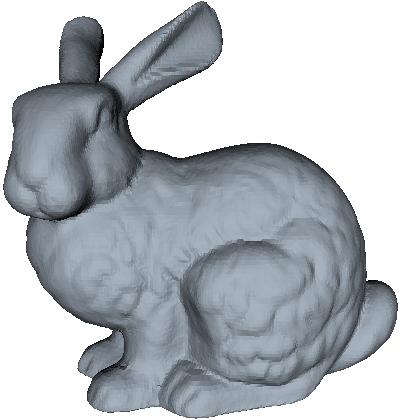
\includegraphics[width=2.5in]{images/ch2/bunny}
                \caption{original}
                \label{fig:bunnyOrigAA}
        \end{subfigure}
        \begin{subfigure}[b]{2.5in}
                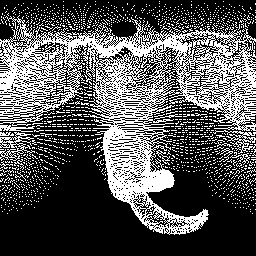
\includegraphics[width=2.5in]{images/ch2/spherical2DMap}
                \caption{transform}
                \label{fig:bunnySPTed}
        \end{subfigure}%
        \caption{The Spherical Map Transform.}
       \label{fig:smtExample}
\end{figure}


Equation \ref{eqn:invLPVVF} is a vector valued function with three separate functions for the x, y and z axis components. These functions are found in equation \ref{eqn:invLPFuncs}. The x-axis function $Ray_x(x,y,r)$ is used together with the $Ray_y(x,y,r)$ and $Ray_z(x,y,r)$ functions to form a spherical transform. The reduction in dimension is achieved by summing the components which share x and y coordinates but have different $r$ (radius) values. In these equations the 3D volume $Vol$ has a width, height and depth of $N$ whilst the output image $Im$ has a width and height of $M$. \\


\begin{equation} \label{eqn:invLPFuncs}
\begin{split}
Ray_x(x,y,r) & = r \times cos\left(\frac{360x}{M}\right)sin\left(\frac{180y}{M}\right)  + \frac{N}{2} \\
Ray_y(x,y,r) & = r \times cos\left(\frac{180y}{M}\right) + \frac{N}{2} \\
Ray_z(x,y,r) & = r \times sin\left(\frac{360x}{M}\right)sin\left(\frac{180y}{M}\right) + \frac{N}{2}
\end{split}
\end{equation}

\begin{equation} \label{eqn:invLPVVF}
Ray(x,y,r) = [Ray_x(x,y,r), Ray_y(x,y,r), Ray_z(x,y,r)]^T
\end{equation}

\begin{equation} \label{eqn:smtUpdate}
Im_{x,y} = \sum_{r=1}^{(2^{-1}N)^{1.5}}{Vol(Ray(x,y,r))} 
\end{equation}

In the Log-Spherical transform described in section \ref{Sec:RoteZoomingSection} re-arranges the rotation and scale transforms along two axis, the third axis retains information and increases the accuracy of the solution. By reducing the other axis from size $N$ to the average value (size 1) information is lost, however computational complexity is reduced by an entire dimension. This is a complexity/performance trade off. Computational complexity may be afforded given input data contains relatively little noise. The output image maps 3D y-axis rotation to 2D x-axis translation. \\


This process essentially sums up the values along a given ray defined by scaling spherical coordinates and adding up the values intersecting the ray. The resulting image, maps 3D y-axis rotation to 2D x-axis translation. Once two 3D frame volumes $V_a$ and $V_b$ are transformed into their corresponding spherical-map domain $SM_a$ and $SM_b$ respectively, the two may be phase correlated to measure the x-axis translation separating them. This x-axis translation may then be mapped directly to the rotational angle separating the two input 3D camera frames. The relationship may be computed as $\frac{360x}{M}$ where $x$ is the x-axis translation and $M$ is the width and height of the spherical map domain image. \\


\subsubsection{Projection-map transform}
\label{sec:PMTramsform}

The Projection-map transform is similar to an orthogonal projection of the volume along a particular axis. Instead of simply projecting the closest point as done in projections for visualization purposes, the sum of values computed along the ray is used for representation. Figure \ref{fig:pmtExample} shows an example model (Figure \ref{fig:bunnyOrigAA2}) and three Projection-map transformations of the model along three different axes (Figures \ref{fig:xaxPMDOM}, \ref{fig:yaxPMDOM} and \ref{fig:zaxPMDOM}). The Projection-map transform is described here in terms of an output Projection-map image $Im$ and an input 3D volume frame $Vol$, which may be input from a sensor or software system which is able to generate 3D frames of the environment. Each pixel in $Im$ has its value defined mathematically as the summation of values along a particular axis given the x,y coordinates. The Projection-map x-axis transform and the Projection-map z-axis transform are defined in equations \ref{eqn:xPMT} and \ref{eqn:zPMT} respectively. \\

\begin{figure}[!htb]
        \centering
        \begin{subfigure}[b]{1.5in}
                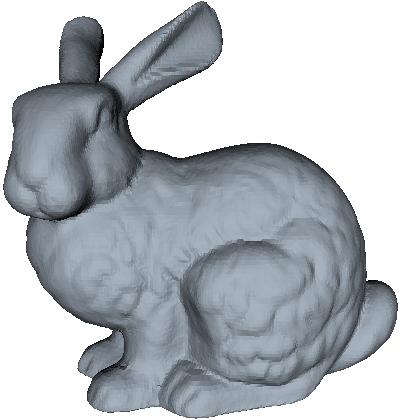
\includegraphics[width=1.5in]{images/ch2/bunny}
                \caption{original}
                \label{fig:bunnyOrigAA2}
        \end{subfigure}%
        \begin{subfigure}[b]{1.5in}
                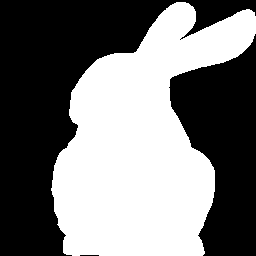
\includegraphics[width=1.5in]{images/methodology/FVR/xaxis}
                \caption{X-Axis Projection-Map Domain}
                \label{fig:xaxPMDOM}
        \end{subfigure}
        \begin{subfigure}[b]{1.5in}
                
\includegraphics[width=1.5in]{images/methodology/FVR/yaxis}
                \caption{Y-Axis Projection-Map Domain}
                \label{fig:yaxPMDOM}
        \end{subfigure}%
        \begin{subfigure}[b]{1.5in}
                
\includegraphics[width=1.5in]{images/methodology/FVR/zaxis}
                \caption{Z-Axis Projection-Map Domain}
                \label{fig:zaxPMDOM}
        \end{subfigure}
        \caption{The Projection-Map Transform.}
       \label{fig:pmtExample}
\end{figure}


\begin{equation} \label{eqn:xPMT}
Im(z,y) = \sum_{x=0}^{N}{Vol(x,y,z)}
\end{equation}

\begin{equation} \label{eqn:zPMT}
Im(x,y) = \sum_{z=0}^{N}{Vol(x,y,z)}
\end{equation}

In these equations the Projection-map transform along the x-axis is computed via summing up values along the x-axis in the input 3D frame. In this way, any 3D z-axis translation in $Vol$ corresponds to 2D x-axis translation in the output image $Im$. Additionally any y-axis translation in the input 3D frame $Vol$ is mapped to a corresponding y-axis translation in the output 2D Projection-map domain $Im$. If both the width and height of the output image $Im$ is equal to the width, height and depth of the input 3D frame then the relationship is a $1:1$ mapping between 3D z-axis translation and 2D x-axis translation as well as 3D y-axis translation to 2D y-axis translation. \\

The corresponding z-axis Projection-map transform sums up values along the z-axis. Here, 3D y-axis translations within the original 3D frame also produce 2D y-axis translations in the output Projection-map domain. However, all x-axis translations occurring within the 3D frame domain are mapped to 2D x-axis translations in the output Projection-map domain image $Im$. \\

Given both of these Projection-map transforms, the 3D translation separating two 3D frames may be registered with respect to 3D translation. This 3D translation also has an inverse relationship to the camera location separation between the two frames. Both 3D frames are transformed into the z-axis Projection-map domain. By phase correlating these domains, both the x and y axis translation may be retrieved which map directly to the 3D translation x and y coordinates separating the input frames. The 3D z-axis translation may be computed by transforming both frames into the x-axis Projection-map domain. Once the two Projection-map domains are phase correlated, the x-axis translation separating the domains can be mapped directly to the corresponding z-axis translation separating the two input 3D frames. In total, using $2 \times$ Projection-map transforms and $1 \times$ 2D phase correlation method, the 3D translation parameters separating two 3D frames may be computed. \\

\subsubsection{Performance Analysis}

To assess the efficiency gain between the Fast Fourier Volume Registration method over the original FVR method, the computational complexity of the FVR is assessed. The computational complexity is dependent on two factors: the size of the input depth map $W \times H$ and the width/height/depth of the 3D volumes used in the volume registration procedure. Since the computational complexity is fixed no matter the input data (depending only on the sizes specified by the user), this method is considered a closed form solution. \\

The FVR method makes use of several sub-procedures including: 2 $\times$ 3D projections (of the depth frame to a 3D volume frame), 2 $\times$ Hanning window filters, 2 $\times$ 3D FFTs, 2 $\times$ element-wise Log filters, 2 $\times$ Log-spherical transforms, 2 $\times$ 3D phase correlation processes and 2 $\times$ linear transformations. The 3D phase correlation method makes use of several sub-procedures including: 3 $\times$ 3D FFTs, 1 $\times$ spectra multiplication and 1 $\times$ 3D peak finding operation. The number of operations required by each of these methods are listed in table \ref{table:complexities}. \\


\begin{table}[ht]
\centering
\caption{Complexities for given Procedures}
\scalebox{0.75}{
\begin{tabular}{cc}
\hline
\textbf{Procedure} & \textbf{Complexity}\\ \hline
3D Projection & $14WH$ \\
Hanning window & 26 (GPGPU)\\
3D FFT & $N^3\log{N^3}$ (GPGPU)\\
Log & 3 (GPGPU) \\
Log-Spherical & 58 (GPGPU)\\
Multiplying Spectra & 15 (GPGPU)\\
Geometric Transform & 30 (GPGPU)\\
3D Peak Search & $2N^3$\\
3D Phase Correlation & $3N^3\log{N^3} + 2N^3 + 44$\\
\\
\end{tabular}}
\\
\label{table:complexities}
\end{table}


Summing these operations whilst scaling them by the number of times they are used gives the total complexity for the FVR method. This complexity is given in equation \ref{eqn:FULLPERFORMANCE}. The complexity of the 3D phase correlation procedure adds up to the complexity shown in equation \ref{eqn:PCFULLPERFORMANCE}. \\

\begin{equation} \label{eqn:FULLPERFORMANCE}
8N^3\log{N^3} + 4N^3 + 28WH + 322
\end{equation}

\begin{equation} \label{eqn:PCFULLPERFORMANCE}
3N^3\log{N^3} + 2N^3 + 15
\end{equation}


The full complexity of the FVR method (equation \ref{eqn:FULLPERFORMANCE}) is next compared to the performance of the FFVR method to assess performance gain. The FFVR methods makes use of several of the procedures found in Table \ref{table:complexities} and several others. These include: 2 $\times$ 3D FFTs, 2 $\times$ Spherical-Map transforms, 3 $\times$ 2D phase correlation procedures, 1 $\times$ 3D geometric transform and 4 $\times$ Projection-Map transforms. The 2D phase correlation method makes use of several sub-procedures including: 3 $\times$ 2D FFTs, 1 $\times$ spectra multiplication and 1 $\times$ 2D peak finding operation. Table \ref{table:complexities2} cites the complexities for the additional operations including: Spherical-Map transform, Projection-Map transform, 2D Peak finding, 2D FFT and 2D phase correlation (made up of multiple sub-procedures). \\



\begin{table}[!htb]
\centering
\caption{Complexities for given Procedures}
\label{table:complexities2}
\scalebox{0.75}{
\begin{tabular}{cc}
\hline
\textbf{Procedure} & \textbf{Complexity}\\ \hline
Spherical-Map Transform & 45 (GPGPU) \\
Projection-Map Transform & 1 (GPGPU) \\
2D Peak Search & $2N^2$ \\
2D FFT & $N^2\log{N^2}$ (GPGPU) \\
2D Phase Correlation & $3N^2\log{N^2} + 2N^2 + 15$ (GPGPU) \\
\\
\end{tabular}}
\\
\end{table}

From Figure \ref{fig:PIPELINE3} we can see that the FFVR method is made up of multiple sub-procedures. These include: 2 $\times$ 3D projections, $2 \times$ 3D FFTs, $2 \times$ Spherical-Map transforms, $1 \times$ 3D geometrical transformation, $3 \times$ 2D phase correlations and $4 \times$ Projection-Map transforms. The total complexity is summed for all of these functions and given in equation \ref{eqn:FULLPERF2}. \\

\begin{equation} \label{eqn:FULLPERF2}
2N^3\log{N^3} + 9N^2\log{N^2} + 6N^2 + 28WH + 169
\end{equation}

Figure \ref{fig:perfComp} provides a visualization of the performance improvement which the FFVR method achieves over the original FVR approach. The graph displays the performance of both methods at different volume sizes increasing logarithmically. The FFVR method is around ~1.8 times faster for $64^3$ volumes, ~3.4 times faster for $128^3$ volumes, ~4.1 times faster for $256^3$ volumes and ~4.2 times faster for $512^3$ volumes. This is due to the reduction in the amount of data to process afforded by the novel spherical-map transform and Projection-map transform methods.

\begin{figure}[!htb]
\centering
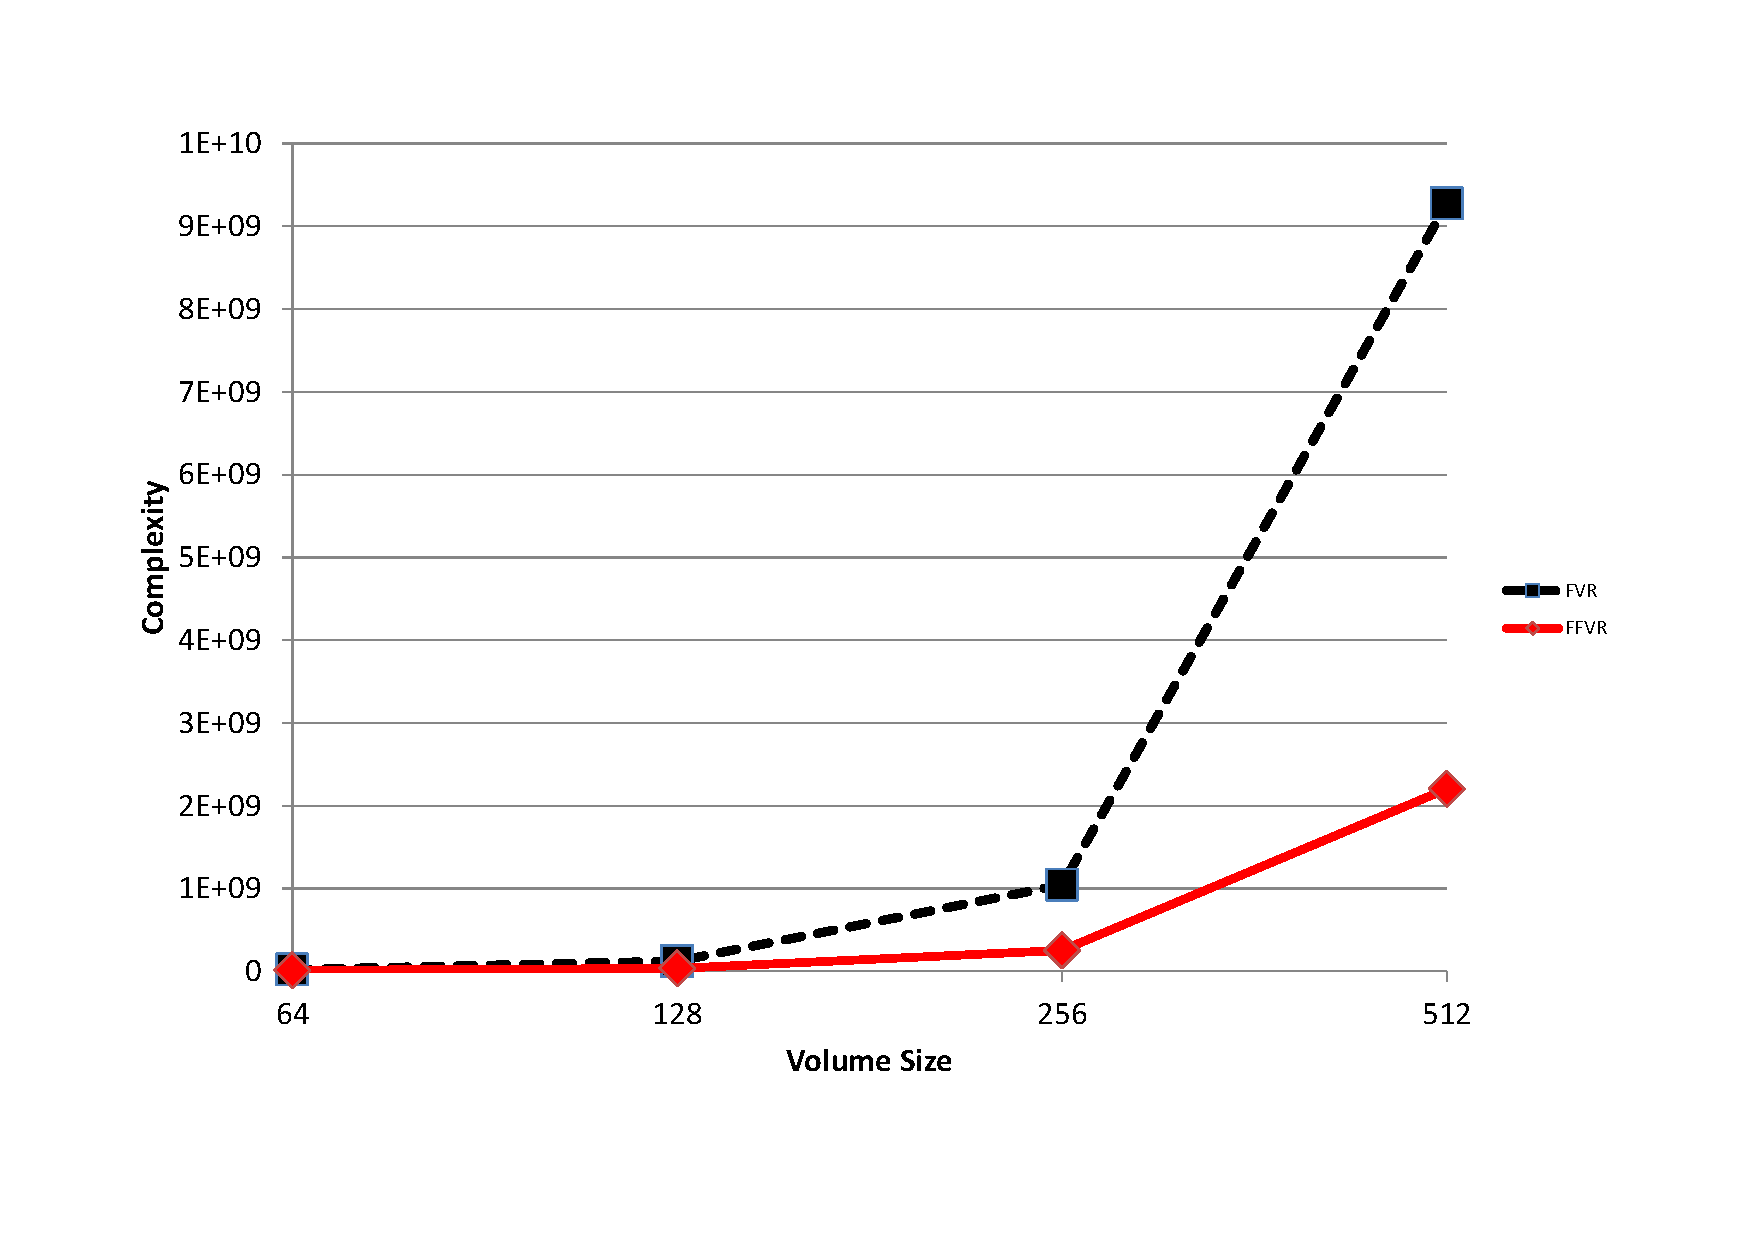
\includegraphics[width=4.0in]{images/methodology/FVR/performanceImprovement}
\caption{Comparison of performance between FVR and FFVR.}
\label{fig:perfComp}
\end{figure}

\subsubsection{Performance Comparison}

In this section, the computational complexities of the FVR related techniques are compared with common algorithms used for 3D reconstruction from the literature. These include: 2D/3D Feature Matching (SURF/SIFT) with RANSAC, PCA, and ICP. These algorithms are compared with the complexity of the FVR, FFVR and FVR-3D (Note: the complexity of MVVR is similar to FVR). Here we use $N$ to represent volume size, for example the FVR based methods usually use a volume of size $N^3$. $W$ is used to describe the size of images processed (used to describe the number of pixels in a $W\times W$ image, projected into a $W\times W$ 3D point cloud). \\


First, the two feature matching methods SIFT and SURF are evaluated. The complexity evaluation of SIFT was taken from work by Vinukonda \cite{Vinukonda11Study} whilst the complexity of SURF was computed based on a public implementation found at \url{https://github.com/lukes611/phdThesis}. The complexity of SIFT is based on the image size $W$, the Gaussian filter size $w$ (typically 5), the number of octaves $s$ (3 are used in experiments), the fraction of extrema in the image $\alpha$ (found to be approximately 6\%), the fraction of extrema which are features $\beta$ (found to be approximately 35\%), the number of additional features found $\gamma$ (found to be approximately 0.04\%) and the size of the descriptor neighbourhood $x$ (typically 8). \\


The complexity of finding SIFT features and computing a SIFT descriptor for an image was found to be,

\begin{equation} \label{eqn:SIFT_PERF}
W^2(s(4w^2 + 100\alpha + 156) + 1520x^2(\alpha \beta + \gamma))
\end{equation}

By plugging in the usual values (equation \ref{eqn:SIFT_PERF_FINAL}), we can form a computational cost as a function of $W$ and variables $\alpha$, $\beta$ and $\gamma$, the variables representing the fraction of pixels which are features.

\begin{equation} \label{eqn:SIFT_PERF_FINAL}
W^2(300\alpha + 768 + 97280(\alpha \beta + \gamma))
\end{equation}

The complexity of SURF is based on several similar factors. Again, $W$ is the image size, $s$ is the number of octaves (3 is the default), $\alpha$ is a scalar (with a default value of 3), and $f$ the fraction of image pixels which are detected as features. Functions which make up the SURF feature detection and descriptor extraction include integral image creation of complexity $W^2 + W$, computation of Hessian feature detection of complexity $\sum_{i=1}^{s} 668(\frac{N}{2^i\alpha})^2$ and the computation of the SURF descriptors of complexity $213434N^2f$. Plugging in default values (equation \ref{eqn:SURF_PERF_FINAL}), the complexity may be formed as a function of the image size, $W$ and the percentage of pixels found to be features $f$.

\begin{equation} \label{eqn:SURF_PERF_FINAL}
W^2 + W + N^2(1972.688 + 213434f)
\end{equation}

The complexity of RANSAC was also analysed. Based the implementation used to compute camera pose from feature matches and corresponding 3D points, the complexity is dependent on $W$ the image size, $I$ the number of iterations (we use 500) and $f$ the fraction of pixels which are matched features. The total complexity is given in equation \ref{eqn:RANSAC_PERF_FINAL}.

\begin{equation} \label{eqn:RANSAC_PERF_FINAL}
134IN^2f
\end{equation}

Therefore, the total complexities of SURF + RANSAC and SIFT + RANSAC are given in equations \ref{eqn:SURFRANSAC_PERF_FINAL} and \ref{eqn:SIFTRANSAC_PERF_FINAL} respectively.


\begin{equation} \label{eqn:SURFRANSAC_PERF_FINAL}
W^2 + W + N^2(1972.688 + 213434f) + 134IN^2f
\end{equation}

\begin{equation} \label{eqn:SIFTRANSAC_PERF_FINAL}
W^2(300\alpha + 768 + 97280(\alpha \beta + \gamma)) + 134IN^2(\alpha \beta + \gamma)
\end{equation}


The complexity of the 3D extension of the SIFT feature matching + RANSAC method  is shown in equation \ref{eqn:SIFT3DRANSAC_PERF_FINAL}, where $N^3$ is the volume size used to project the 3D data into.

\begin{equation} \label{eqn:SIFT3DRANSAC_PERF_FINAL}
N^3(1968 + 300\alpha + 41040(\alpha \beta + \gamma)) + 134IN^3(\alpha \beta + \gamma)
\end{equation}

The complexity of the PCA method was taken from \cite{Johnstone04Sparse}. It is a function of $W$ (again where the number of pixels in the image is $W^2$) and $p = 3$, the dimensionality of the 3D points. The complexity was found to be $p^2W^2+p^3$, plugging in 3 for $p$ gives the complexity as a function of $W$ provided in equation \ref{eqn:PCA_PERF_FINAL}.

\begin{equation} \label{eqn:PCA_PERF_FINAL}
9W^2 + 27
\end{equation}

Finally the complexity of ICP is described. The complexity of ICP in the context of pose estimation is based on the complexity of (i) computing the K Nearest Neighbours (KNN) algorithm between point clouds ($3W^2f$), (ii) computing the least squares optimal pose based on the matches ($16W^2f + 96$), and (iii) testing the computed pose $21W^2f$. Here, $W$ is the image size and $f$ is the fraction of projected pixels used in the ICP algorithm. This is performed up to 500 times leading to the complexity in equation \ref{eqn:ICP_PERF_FINAL}.

\begin{equation} \label{eqn:ICP_PERF_FINAL}
1008W^8f^3 + 6048W^4f^2
\end{equation}

\begin{table}[!t]
\centering
\caption{Algorithm Complexities}
\begin{tabular}{cc}\hline
\textbf{Algorithm} & \textbf{Complexity}\\ \hline
FM2D + RANSAC & $W^2 + W + W^2(1972.688 + 213434f) + 134IW^2f$\\
FM3D + RANSAC & $N^3(1968 + 41040f) + 134IN^3f$\\
PCA & $9W^2 + 27$\\
ICP & $1008W^8f^3 + 6048W^4f^2$\\
FVR & $8N^3\log{N^3} + 4N^3 + 322$\\
FFVR & $2N^3\log{N^3} + 9N^2\log{N^2} + 6N^2 + 169$\\
FVR-3D & $8N^3\log{N^3} + 4N^3 + 349 + 9W^2$\\
\\
\end{tabular}
\\[10pt]
\label{table:ALG_COMPLEX_TBL}
\end{table}

The complexities for each of the algorithms mentioned are shown in Table \ref{table:ALG_COMPLEX_TBL}. Figure \ref{fig:COMPLEX_COMP_CHART} compares complexity as a function of percentage of pixels used as features. In this figure, both ICP and FM-3D were omitted as they had theoretical performances which were so large they skewed the comparison (for perspective, Figure \ref{fig:COMPLEX_COMP_CHART_ALL} includes both ICP and FM3D). In these tests, we used a RANSAC iteration count of 500, image sizes of $1024^2$ and volume sizes of $256^3$. The RANSAC iteration count was chosen as it worked well in experiments, the image sizes were chosen to be HD and the volume size was chosen based on the experiments performed using the FVR based algorithms. Comparing these results, FM2D has the largest complexity. FVR and FVR-3D had essentially the same complexity and FFVR was found to be slightly faster than these, as it was designed to be. PCA is the simplest algorithm and the fastest here. Both ICP and FM-3D had complexities which increased exponentially as the percentage of pixels increased, whilst FM2D increased linearly. PCA and the FVR based methods have flat complexities which do not vary with the number of features used since they use the entire point cloud or volume. \\


\begin{figure}
        \centering
        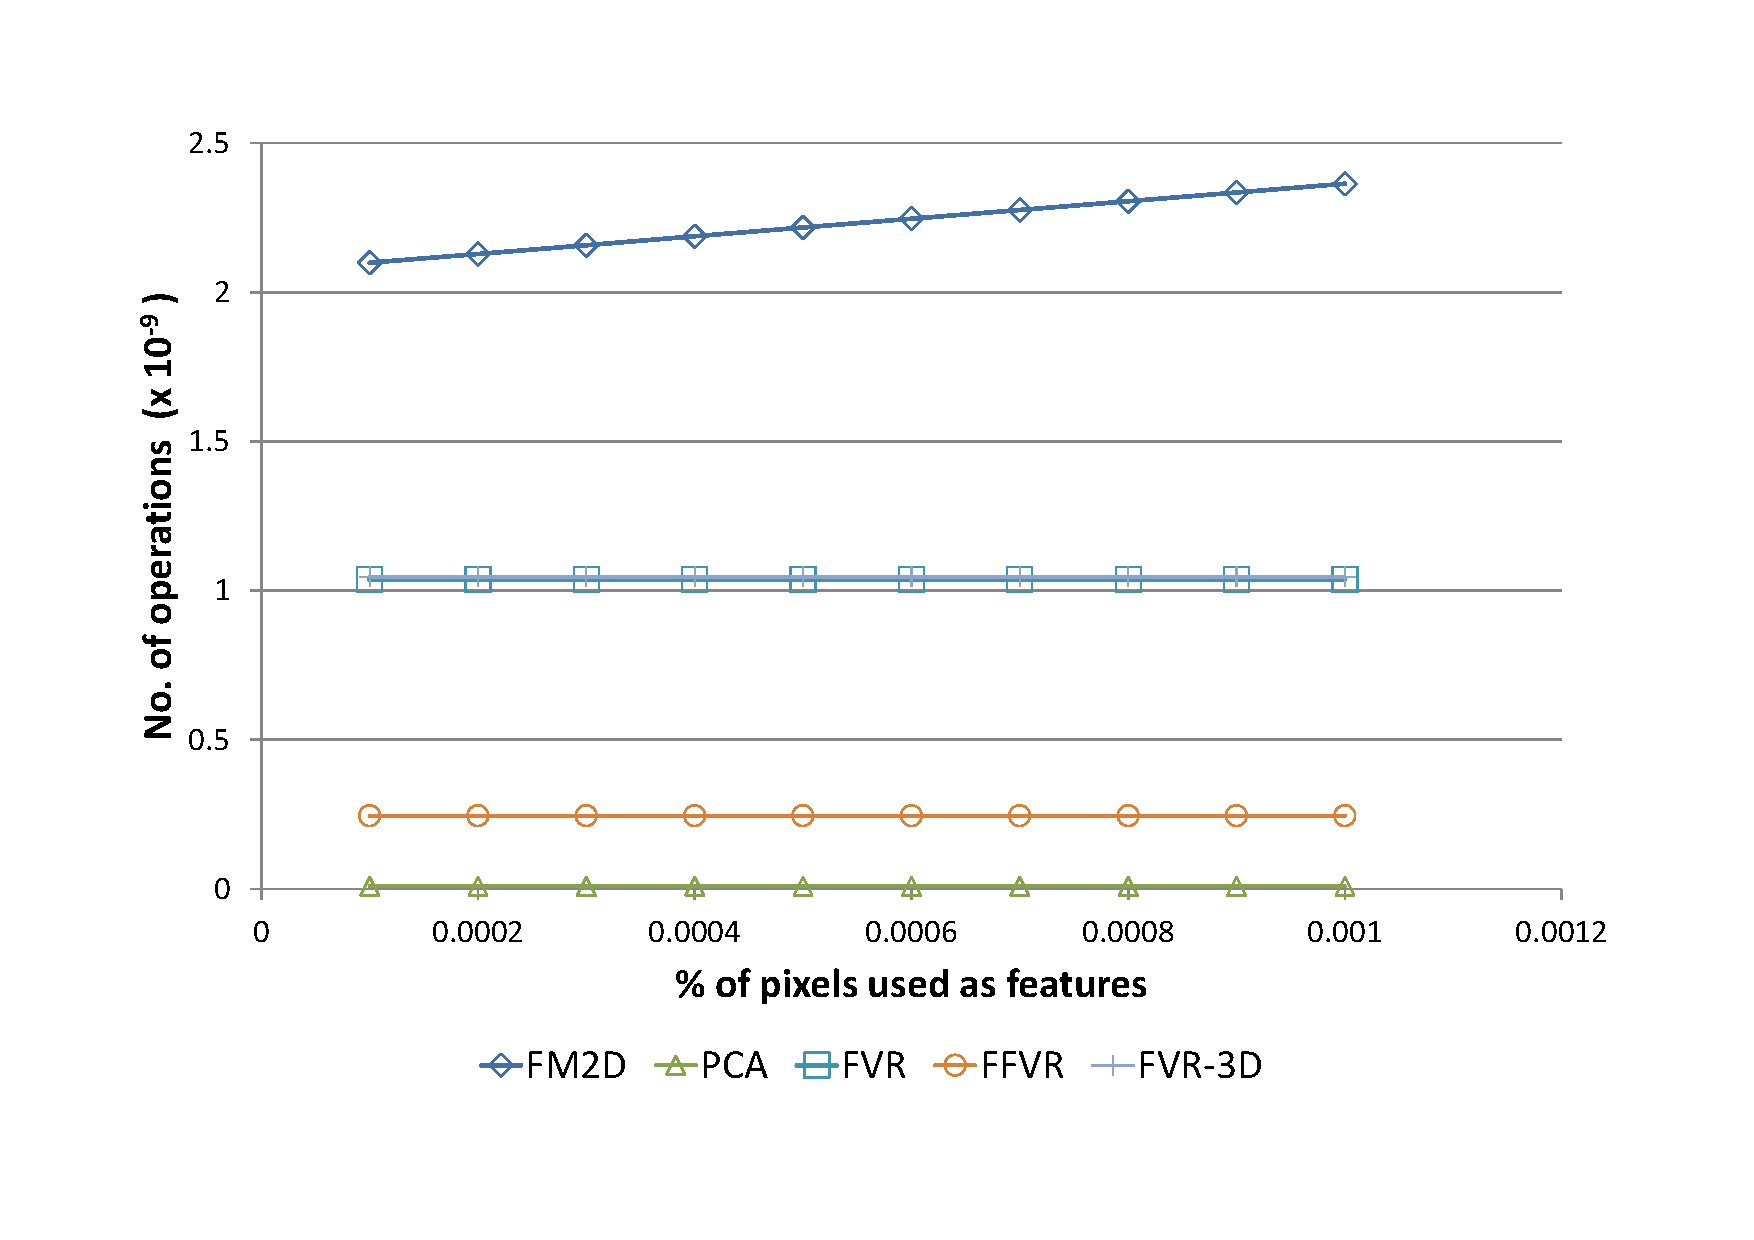
\includegraphics[width=5.0in]{images/theoreticalSpeedComparison}
        \caption{Theoretical Complexity Comparison}
        \label{fig:COMPLEX_COMP_CHART}
\end{figure}


\begin{figure}
        \centering
        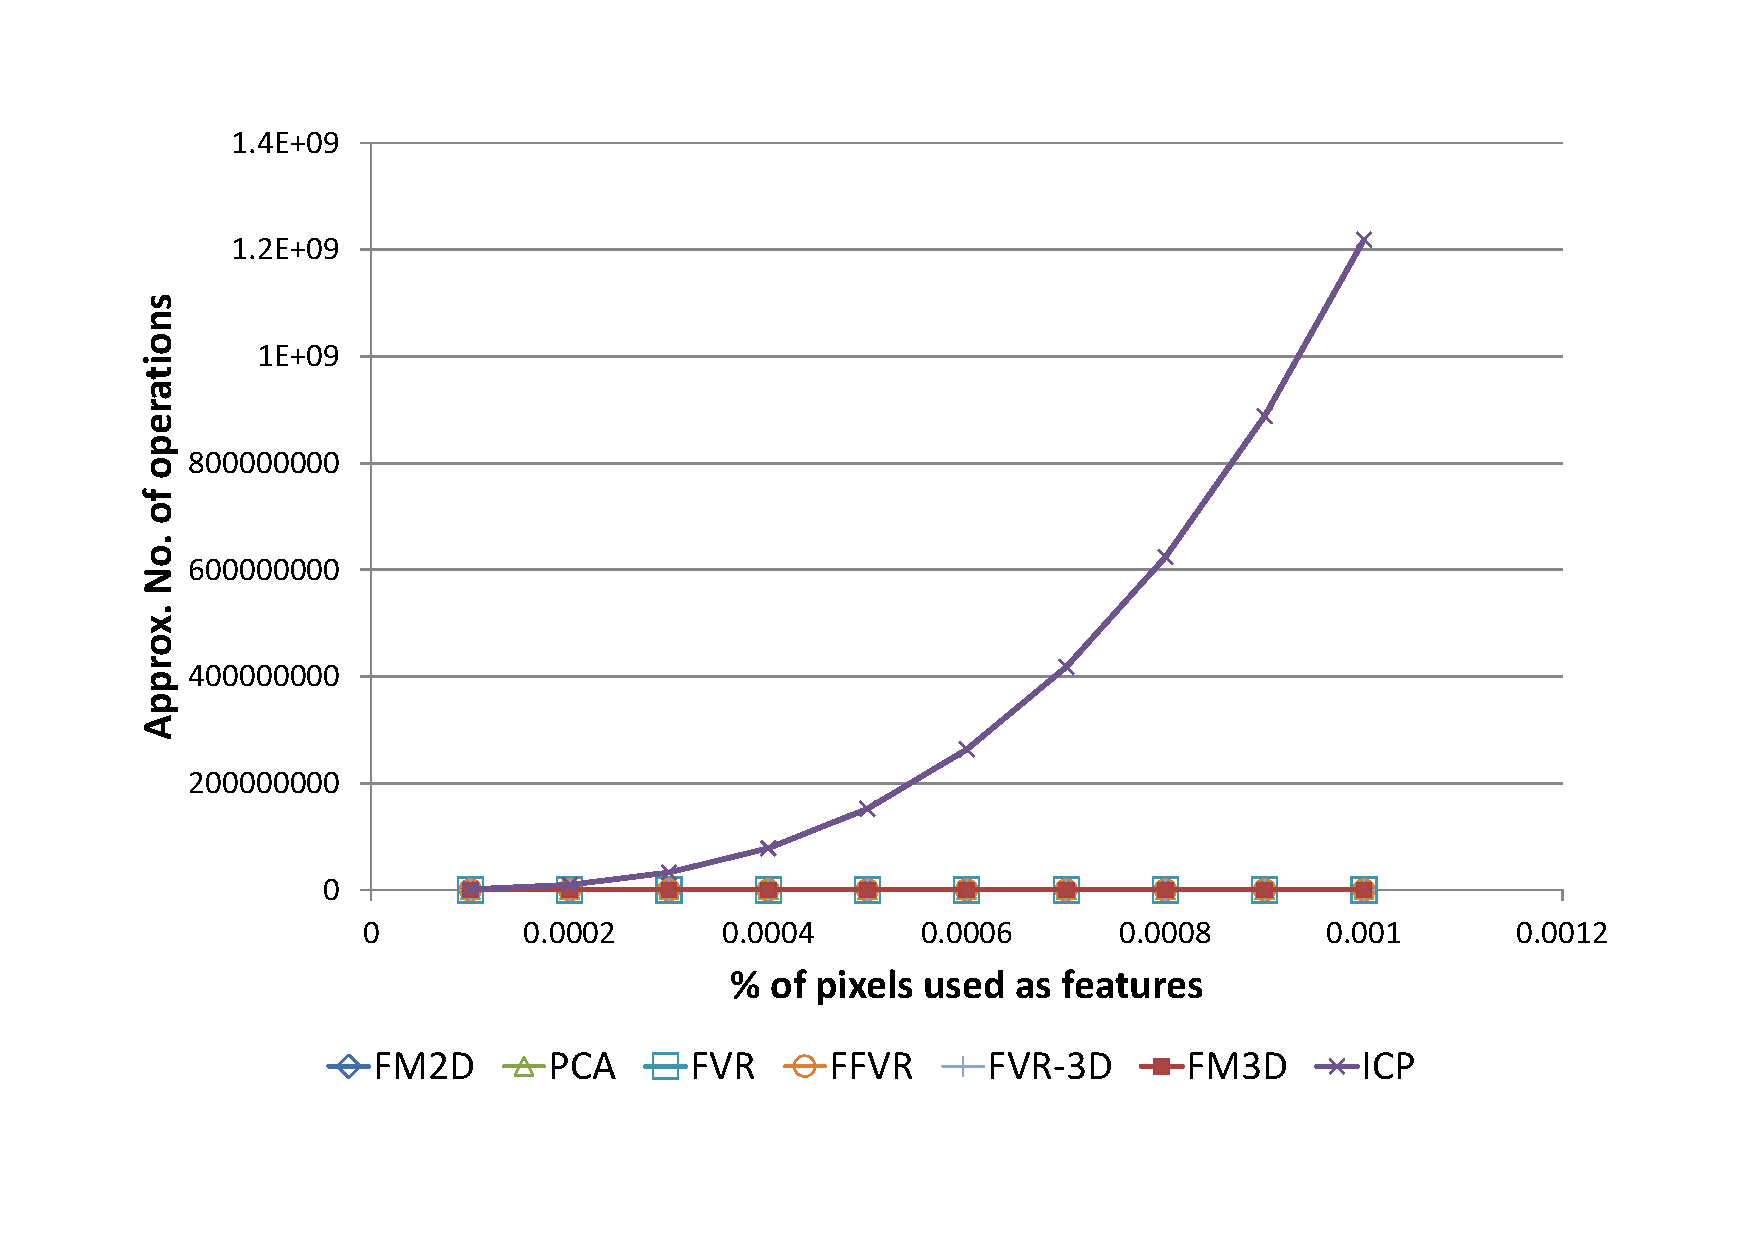
\includegraphics[width=5.0in]{images/theoreticalSpeedComparisonAll}
        \caption{Theoretical Complexity Comparison (Including FM3D and ICP)}
        \label{fig:COMPLEX_COMP_CHART_ALL}
\end{figure}
